\documentclass[ucs]{beamer}\usepackage[]{graphicx}\usepackage[]{color}
%% maxwidth is the original width if it is less than linewidth
%% otherwise use linewidth (to make sure the graphics do not exceed the margin)
\makeatletter
\def\maxwidth{ %
  \ifdim\Gin@nat@width>\linewidth
    \linewidth
  \else
    \Gin@nat@width
  \fi
}
\makeatother

\definecolor{fgcolor}{rgb}{0.345, 0.345, 0.345}
\newcommand{\hlnum}[1]{\textcolor[rgb]{0.686,0.059,0.569}{#1}}%
\newcommand{\hlstr}[1]{\textcolor[rgb]{0.192,0.494,0.8}{#1}}%
\newcommand{\hlcom}[1]{\textcolor[rgb]{0.678,0.584,0.686}{\textit{#1}}}%
\newcommand{\hlopt}[1]{\textcolor[rgb]{0,0,0}{#1}}%
\newcommand{\hlstd}[1]{\textcolor[rgb]{0.345,0.345,0.345}{#1}}%
\newcommand{\hlkwa}[1]{\textcolor[rgb]{0.161,0.373,0.58}{\textbf{#1}}}%
\newcommand{\hlkwb}[1]{\textcolor[rgb]{0.69,0.353,0.396}{#1}}%
\newcommand{\hlkwc}[1]{\textcolor[rgb]{0.333,0.667,0.333}{#1}}%
\newcommand{\hlkwd}[1]{\textcolor[rgb]{0.737,0.353,0.396}{\textbf{#1}}}%

\usepackage{framed}
\makeatletter
\newenvironment{kframe}{%
 \def\at@end@of@kframe{}%
 \ifinner\ifhmode%
  \def\at@end@of@kframe{\end{minipage}}%
  \begin{minipage}{\columnwidth}%
 \fi\fi%
 \def\FrameCommand##1{\hskip\@totalleftmargin \hskip-\fboxsep
 \colorbox{shadecolor}{##1}\hskip-\fboxsep
     % There is no \\@totalrightmargin, so:
     \hskip-\linewidth \hskip-\@totalleftmargin \hskip\columnwidth}%
 \MakeFramed {\advance\hsize-\width
   \@totalleftmargin\z@ \linewidth\hsize
   \@setminipage}}%
 {\par\unskip\endMakeFramed%
 \at@end@of@kframe}
\makeatother

\definecolor{shadecolor}{rgb}{.97, .97, .97}
\definecolor{messagecolor}{rgb}{0, 0, 0}
\definecolor{warningcolor}{rgb}{1, 0, 1}
\definecolor{errorcolor}{rgb}{1, 0, 0}
\newenvironment{knitrout}{}{} % an empty environment to be redefined in TeX

\usepackage{alltt}     	% document art 
\usepackage[utf8x]{inputenc}  		% support for unicode-signs
\usepackage[T1]{fontenc}      		% support for European signs
\usepackage[scaled=.90]{helvet}  	% font: Helvetica
\usepackage{mathptmx}            	% for maths writings
\usepackage{courier}             	% passende Monospaced-Schriftart
\usepackage{tikz}				          % for placing pictures on an absolute position
\usepackage{graphicx}
\usepackage{xcolor,colortbl}
\definecolor{babyblueeyes}{rgb}{0.63, 0.79, 0.95}
%for colored tables 
\newcount\colveccount
\newcommand*\colvec[1]{
        \global\colveccount#1
        \begin{pmatrix}
        \colvecnext
}
\def\colvecnext#1{
        #1
        \global\advance\colveccount-1
        \ifnum\colveccount>0
                \\
                \expandafter\colvecnext
        \else
                \end{pmatrix}
        \fi
}
%%
%\mode<presentation>{
\usetheme{Darmstadt}   	 	% slides style (Franfkurt, Berlin)
\usecolortheme{dove}     	% colour scheme (seahorse)
\setbeamertemplate{navigation symbols}{}%remove navigation symbols
%} 
%%% information about presentation %%%%%%%%%%%%%%%%%%%%%%%%%%%%%%%%%%%
\IfFileExists{upquote.sty}{\usepackage{upquote}}{}
\begin{document}
\title{Main Points of: Imagining and Imaging: Creating
a New Model World}
\subtitle{\footnotesize{Paul Sch\"afer}}
%\date{\tiny{\today}}
 
%%% document %%%%%%%%%%%%%%%%%%%%%%%%%%%%%%%%%%%%%%%%%
\setbeamercolor{block title}{fg=black!60,
bg= blue!10}
\setbeamercolor{block body}{fg=black!70,
bg= white!10}


% title

\begin{frame}
\titlepage
\end{frame}

\begin{frame}
\frametitle{Outline}
\setbeamercolor{section in toc shaded}{fg=black!70,
bg= black!10}
\setbeamercolor{section in toc}{fg=black!70,
bg= white!10}
\setbeamertemplate{sections/subsections in toc}[sections numbered]
  \tableofcontents
\end{frame}

\section{Languages of Modeling}
\begin{frame}{Conceptual versus Perceptual Space}
\begin{table}
\begin{center}
\begin{tabular}{|l|l|}
\hline
\textbf{Perceptual Space }& \textbf{Conceptual Space}\\ \hline
Artist & Economist \\ \hline
Illustrates & Visualizes \\ \hline
Understanding the Perceptual Space & Concepts and Manipulation\\ \hline

\end{tabular}
\end{center}
\end{table}
\end{frame}


\begin{frame}{Modeling and the Use of Mathematics}
	\begin{itemize}
		\item Mathematical Languages:
	  		\begin{itemize}
	  		\item Use of symbols
	  		\item Manipulation of symbols
	  		\item Rules for the manipulation of symbols given by the language and the model
	  		\end{itemize}
	 \item Sentences Math and Diagrams
	 	\begin{itemize}
	 		\item Math is closer to sentences than to diagrams
	 		\item Math and sentences express ideas in temporal or logical relations
	 		\item Diagrams express ideas in spatial relations
	 	\end{itemize}
	\end{itemize}
\end{frame}

\section{Visualization}
\begin{frame}{The Process of Visualization}
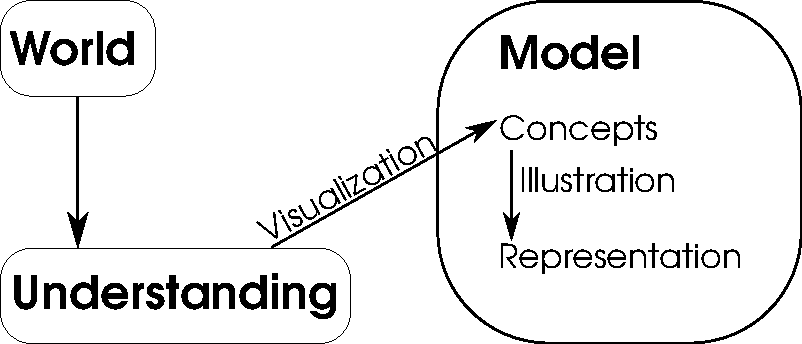
\includegraphics[scale = 0.8]{ImagingImaginingDiagramm.pdf}	
\end{frame}

\section{Newness}
\begin{frame}{Imagining new Concepts}
\begin{itemize}
\item New World with new Concepts
\item Modeling leads to other statements about the World than verbal economics
\item Expressing Models in verbal form needs new words for new concepts
\item The model becomes essential to the text
\end{itemize}
\end{frame}


\section{The History of the Edgeworth Box}
\begin{frame}{Marshall's  first Trade Diagram (1879)}
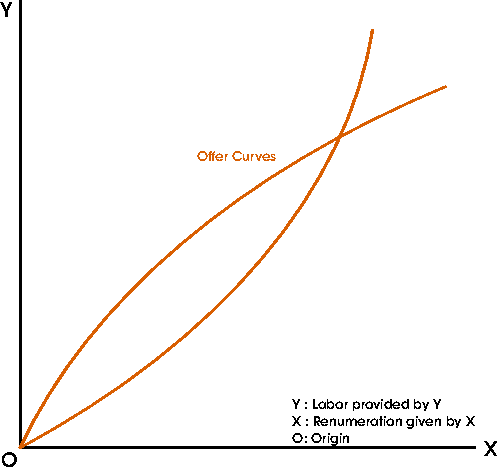
\includegraphics[scale = 0.9]{Marshall.pdf}
\end{frame}

\begin{frame}{The Original Edgeworth Box (1881)}
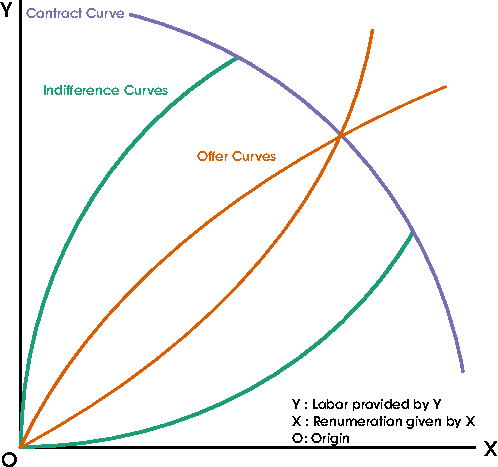
\includegraphics[scale = 0.9]{EdgeworthBox.pdf}
\end{frame}

\begin{frame}{Pareto's "Optimum" Box Diagram (1906)}
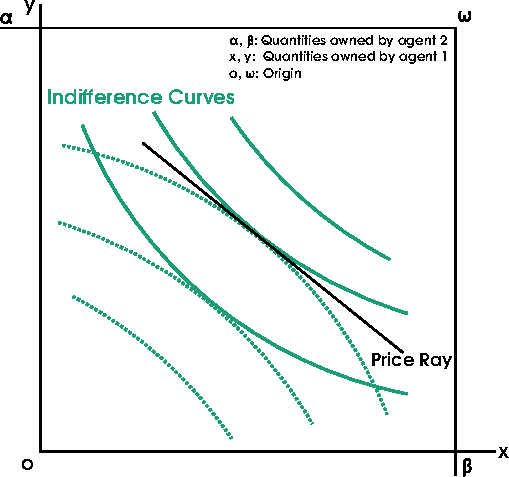
\includegraphics[scale = 0.9]{Pareto.pdf}
\end{frame}

\begin{frame}{Newness and the Edgeworth Box}
\begin{itemize}
\item Marshall's first trade diagram (1879)
	\begin{itemize}
		\item Offer curves
	\end{itemize}
\item The original Edgeworth box (1881) 
	\begin{itemize}
		\item Indifference curves
		\item Contract curve
	\end{itemize}
\item Pareto's "optimum" box diagram (1906)
	\begin{itemize}
		\item Pareto optimality
	\end{itemize}
\end{itemize}
\end{frame}
\end{document}
